\section{Motivation}
\label{section:intro}

Modern interactive web applications aim to 
provide a highly responsive user experience by 
minimising the communication latency between clients and servers. 
Whilst the \textit{HTTP} 
request-response model is 
sufficient for retrieving static assets, 
applying the same 
stateless communication approach for 
interactive use cases 
introduces 
undesirable performance overhead from having to 
frequently set up 
new connections for client-server interactions. 
Developers have since adopted other communication 
transport abstractions over HTTP connections such 
as the WebSockets protocol \cite{WebSocketRFC}
to enjoy low-latency full-duplex 
client-server communication in their applications over 
a single persistent connection. 
Enabling more complex communication patterns caters for 
more interactive use cases, but introduces additional 
concerns to the developer with respect to implementation correctness.

\paragraph{Communication Safety 
in Interactive Web Applications}

Consider a \textit{flight booking service}
between a \trole{Traveller} and a \trole{FlightServer}.
The \trole{Traveller} queries the \trole{FlightServer}
about prices to a particular destination.
If there is still availability, 
the \trole{FlightServer} will \textit{reserve a seat}
responds with the price,
to which the \trole{Traveller} confirms or rejects the purchase;
the latter choice will notify the \trole{FlightServer}
to \textit{release the seat}.
Otherwise, the \trole{FlightServer} notifies the
\trole{Traveller} that all flights are full.
The \trole{Traveller} can proceed to query for another
destination.

We can implement the flight booking service as a web
application.
\trole{FlightServer} can be a web server
running on the \textit{Node.js} JavaScript runtime \cite{nodejs}.
\trole{Traveller} can run on the web browser
as a \textit{single-page application} (SPA) written
in a popular framework like \textit{React.js} \cite{React}.
SPAs feature a single HTML page and dynamically renders
content via JavaScript in the browser.
The \trole{Traveller} connects to the \trole{FlightServer}
using a WebSocket connection and they enjoy
bi-directional communication to execute the flight
booking operations outlined above.
We visualise the interactions in \cref{fig:flightbook}

\begin{figure}[!ht]
\centering
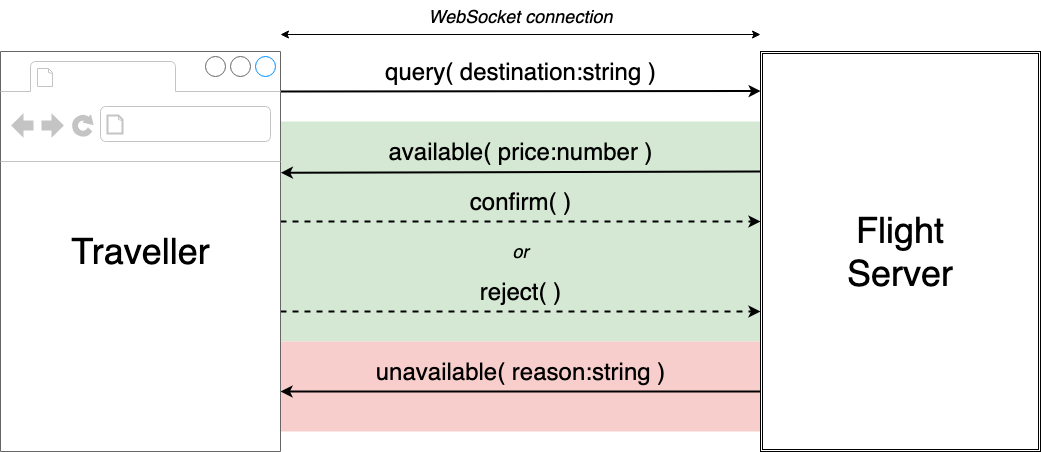
\includegraphics[width=0.7\textwidth]{FlightBookingService}
\captionof{figure}{Message-Passing Architecture of Web-Based 
Flight Booking Service}
\label{fig:flightbook}
\end{figure}

Whilst WebSockets make this web-based implementation possible, 
it introduces the developer to a new family of communication errors
(in addition to the usual testing for application logic correctness), 
even for this simple example:

\begin{itemize}

\item
\textbf{Deadlocks:} how can we prevent both sides waiting for 
each other to respond at the same time?

\item 
\textbf{Communication mismatches:} what if the 
\trole{FlightServer} sends a string to the \trole{Traveller}
who is expecting the price to be a numeric value?

\item
\textbf{Channel linearity:} if the \trole{FlightServer}
takes time to respond to a query from the \trole{Traveller},
what if the \trole{Traveller} sends the same query twice? 
Given that the \trole{FlightServer} reserves a seat on
a ``successful'' query, violating channel linearity
would hold up seats unnecessarily.

\end{itemize}

The complexity of these errors,
which correlate to the complexity of tests 
required against these errors, 
scale with the complexity of the 
communication patterns involved. 
Over-reliance on integration testing
to attempt to expose communication-related bugs 
will also slow the
development process, not to mention that the time 
taken for these
integration tests would scale with the number of roles involved.
A localised, static way for verifying communication correctness
is highly desirable.

\paragraph{Formalising Interactions with
Multiparty Session Types}
\textit{Multiparty Session Types} (MPST) \cite{MPST} 
provide a framework for formally specifying 
a structured communication pattern 
between concurrent processes and 
verifying implementations for 
correctness with respect to the communications aspect. 

By specifying the client-server interactions of 
our flight booking service as a protocol 
and verifying the implementations against 
the protocol for well-formedness, 
MPST theory guarantees well-formed 
implementations to be free from communication errors.

\paragraph{Limitations of State-of-the-Art Session-Typed Web Development}
Existing work \cite{MVU2020,PureScript2019} that 
adapt the MPST framework for web development
acknowledge the limitations of \textit{JavaScript} 
-- the language of the browser --
in providing static type-level guarantees
for communication safety, 
and proceed to use
languages equipped with stronger type systems that 
compile to JavaScript instead.

With respect to the end goal of 
offering developers a development workflow
that provides communication safety guarantees in modern
web programming through multiparty session types,
we observe two main limitations from the state-of-the-art:

\subparagraph{L1: 
Incompatibility with modern web programming practices}

The current state-of-the-art succeeds in statically
providing communication safety guarantees,
but requires the developer to compromise by adapting
to programming paradigms and practices that are not
conventional for modern web programming.
Developers that use \cite{MVU2020} are required
to implement their web applications in a \textit{functional} 
paradigm using the \textit{Links} 
web programming language \cite{LINKS}.
\cite{PureScript2019} also endorses
functional web programming by requiring developers to
write PureScript \cite{PureScript} applications, but also
enforces user interfaces to be written using 
sequential UI frameworks.

PureScript and Links are not interoperable
with the ever-growing universe of JavaScript libraries for
web development.
It is also unclear whether these tools support idiomatic
practices in event-driven programming, such as callbacks
and asynchronous implementations.
Whilst communication safety guarantees provided by
\cite{PureScript2019,MVU2020} are based on
canonical MPST theory, they are not contextualised
for the dynamic web-based environment.
Going back to the flight booking service as an example,
\cite{PureScript2019,MVU2020} do not handle premature
disconnections; if the \trole{Traveller} receives a quote
and closes their browser prematurely and the \trole{FlightServer}
is not notified of this event, 
the reserved seat will not be released.
These compromises limit the usability of the MPST framework
in modern web programming.

\subparagraph{L2: 
Limited expressiveness of communication protocols}

The current state-of-the-art leverage the WebSocket protocol
as the communication transport between roles, which is
simple to reason about and straightforward to relate
to session type theory.
However, WebSocket transport enforces a \emph{server-centric}
network topology, so \cite{PureScript2019,MVU2020}
enforces the same constraint on the range of communication
protocols supported:
server-centric protocols feature exactly one server
role that is involved in all interactions. 

This limits the types set of communication topologies
that can be implemented by session-typed web development
proposals. 
Suppose we extend the flight booking service as follow:
we introduce a \trole{TravelAgent} role, which
runs on the browser; the \trole{Traveller} first asks
for a quote from the \trole{TravelAgent} before 
carrying out the usual interactions with the \trole{FlightServer},
so the \trole{Traveller} can compare between both options.
The current state-of-the-art cannot implement this 
extended flight booking service, as the described
communication interactions is no longer server-centric.